\documentclass[border=10pt]{standalone}
\usepackage{tikz}
\usepackage{amsmath}
\usetikzlibrary{arrows.meta,positioning}

% 与原 MLP 图相同的配色
\definecolor{inFill}{RGB}{183,224,177}
\definecolor{inLine}{RGB}{32,102,32}
\definecolor{hidFill}{RGB}{199,203,243}
\definecolor{hidLine}{RGB}{52,58,143}
\definecolor{outFill}{RGB}{243,199,199}
\definecolor{outLine}{RGB}{143,52,52}
\definecolor{lineC}{RGB}{38,44,110}
% 计算图新增配色：偏置 / 运算符节点
\definecolor{biasFill}{RGB}{255,241,194}
\definecolor{biasLine}{RGB}{171,122,34}
\definecolor{opFill}{RGB}{250,250,250}
\definecolor{opLine}{RGB}{70,70,70}

\begin{document}
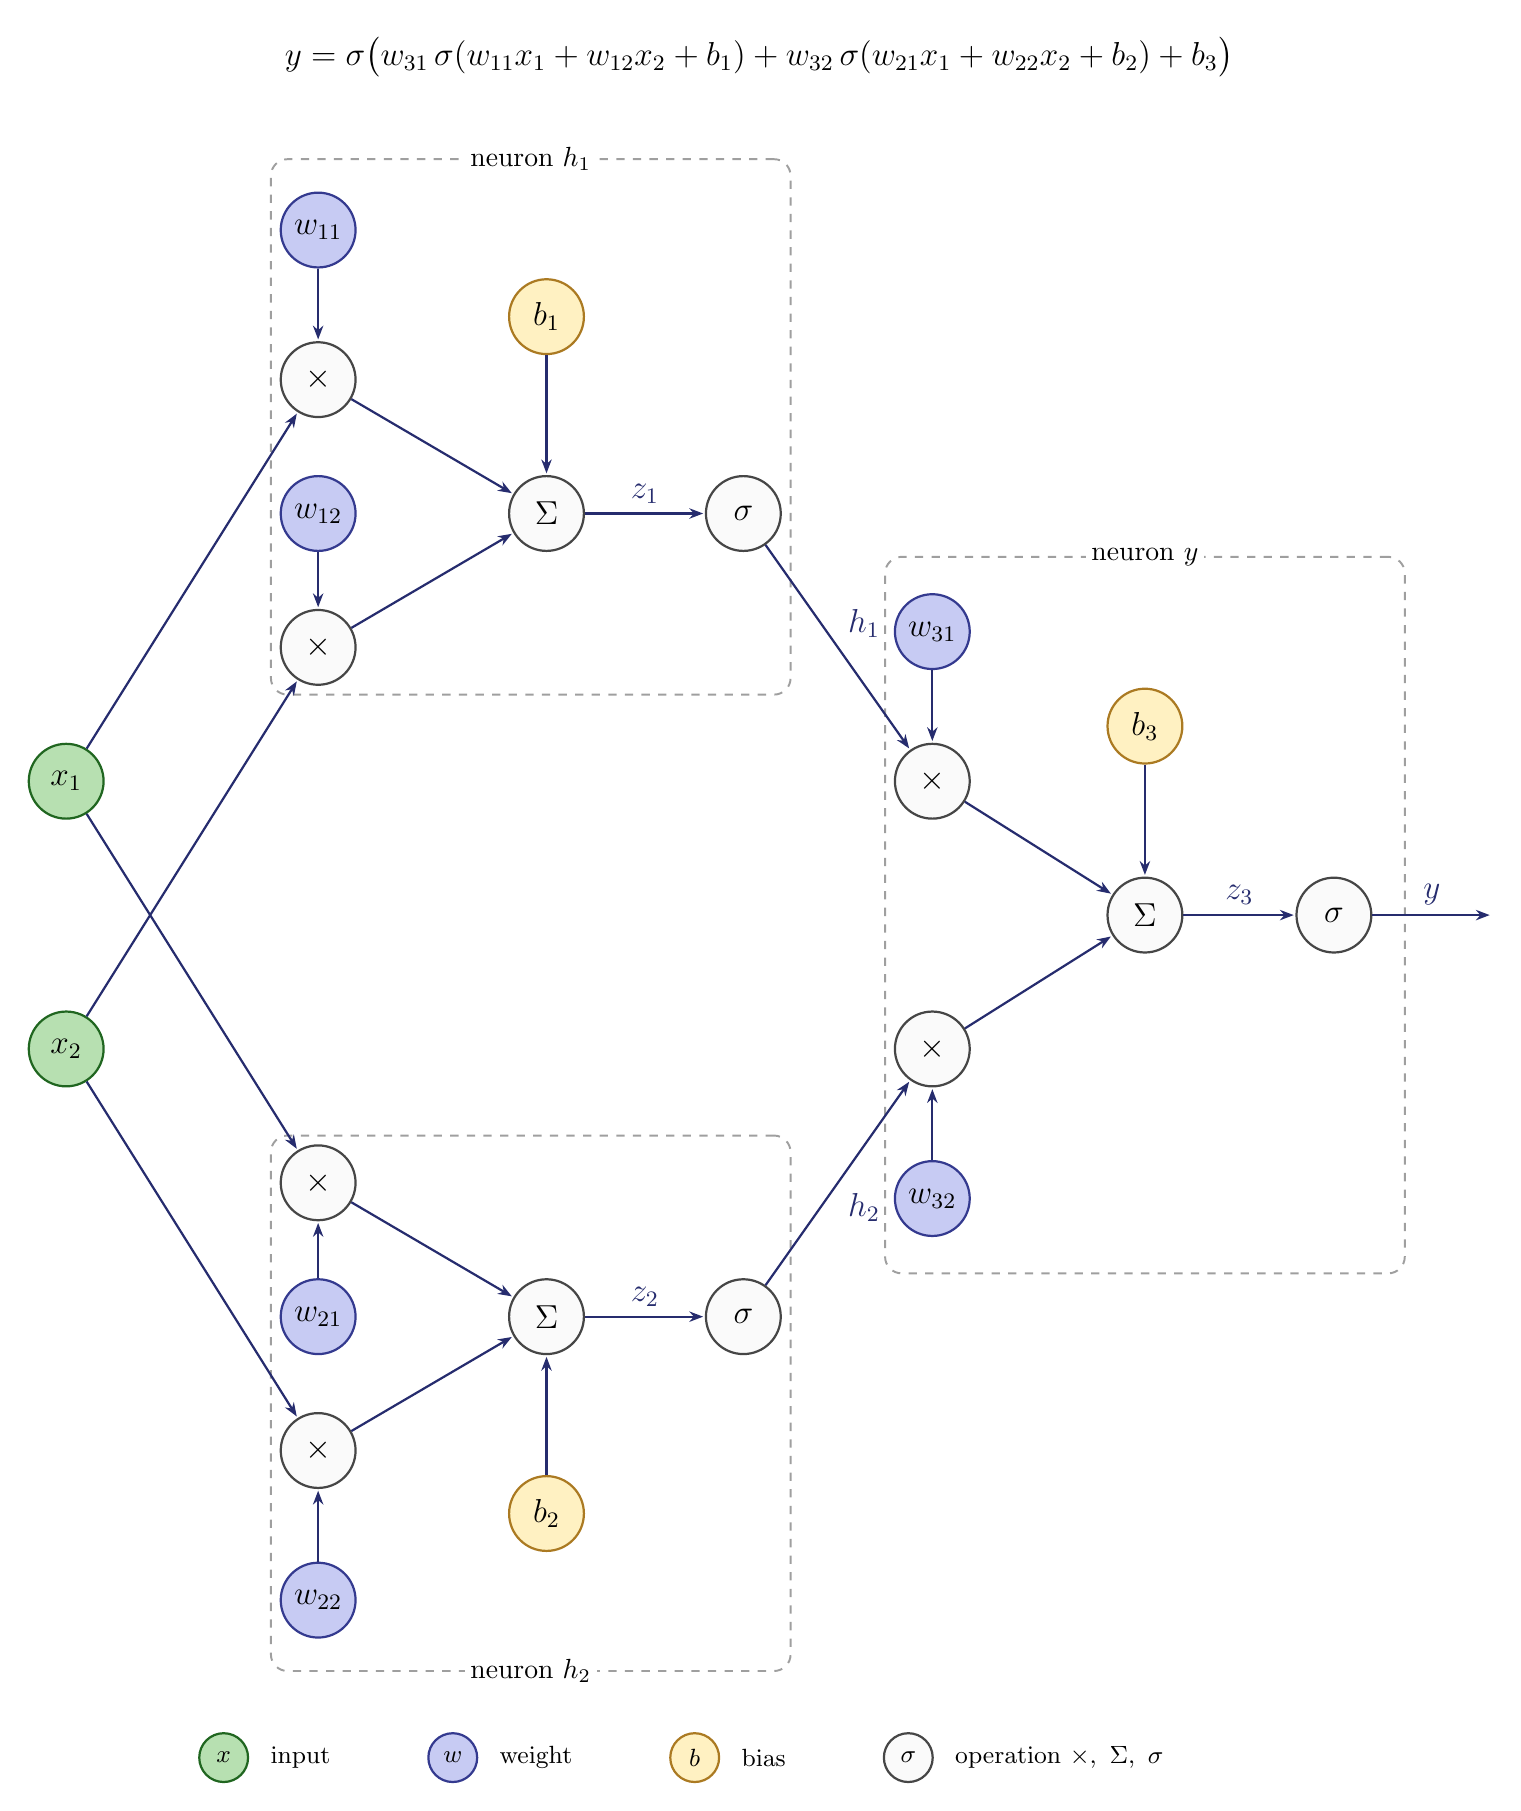
\begin{tikzpicture}[
    >={Stealth[length=5pt]}, line width=0.8pt, font=\large,
    op/.style  ={circle, draw=opLine, fill=opFill, minimum size=0.95cm, inner sep=0pt},
    leaf/.style={circle, minimum size=0.95cm, inner sep=1pt},
    inp/.style ={leaf, draw=inLine, fill=inFill},
    wgt/.style ={leaf, draw=hidLine, fill=hidFill},
    bia/.style ={leaf, draw=biasLine, fill=biasFill},
    arr/.style ={lineC, ->, shorten >=0.6pt},
    nbox/.style={draw=gray!75, line width=0.7pt, dashed, rounded corners=6pt},
  ]

  % ---- 虚线框：每个神经元展开成一个小计算子图 ----
  \node[nbox, minimum width=6.6cm, minimum height=6.8cm] at (5.9, 6.2) {};
  \node[nbox, minimum width=6.6cm, minimum height=6.8cm] at (5.9,-6.2) {};
  \node[nbox, minimum width=6.6cm, minimum height=9.1cm] at (13.7, 0) {};
  \node[fill=white, inner sep=2pt, font=\normalfont] at (5.9, 9.6)   {neuron $h_1$};
  \node[fill=white, inner sep=2pt, font=\normalfont] at (5.9,-9.6)   {neuron $h_2$};
  \node[fill=white, inner sep=2pt, font=\normalfont] at (13.7, 4.55) {neuron $y$};

  % ---- 整张图对应的复合函数 ----
  \node[font=\large] at (8.8,10.9)
    {$y=\sigma\big(w_{31}\,\sigma(w_{11}x_1+w_{12}x_2+b_1)+w_{32}\,\sigma(w_{21}x_1+w_{22}x_2+b_2)+b_3\big)$};

  % ---- 输入 ----
  \node[inp] (x1) at (0, 1.7) {$x_1$};
  \node[inp] (x2) at (0,-1.7) {$x_2$};

  % ---- 第一层：乘法与权重 ----
  \node[op]  (m11) at (3.2, 6.8) {$\times$};
  \node[op]  (m12) at (3.2, 3.4) {$\times$};
  \node[op]  (m21) at (3.2,-3.4) {$\times$};
  \node[op]  (m22) at (3.2,-6.8) {$\times$};
  \node[wgt] (w11) at (3.2, 8.7) {$w_{11}$};
  \node[wgt] (w12) at (3.2, 5.1) {$w_{12}$};
  \node[wgt] (w21) at (3.2,-5.1) {$w_{21}$};
  \node[wgt] (w22) at (3.2,-8.7) {$w_{22}$};

  % ---- 第一层：求和与偏置 ----
  \node[op]  (s1) at (6.1, 5.1) {$\Sigma$};
  \node[op]  (s2) at (6.1,-5.1) {$\Sigma$};
  \node[bia] (b1) at (6.1, 7.6) {$b_1$};
  \node[bia] (b2) at (6.1,-7.6) {$b_2$};

  % ---- 第一层：激活 ----
  \node[op] (a1) at (8.6, 5.1) {$\sigma$};
  \node[op] (a2) at (8.6,-5.1) {$\sigma$};

  % ---- 第二层（输出神经元） ----
  \node[op]  (m31) at (11.0, 1.7) {$\times$};
  \node[op]  (m32) at (11.0,-1.7) {$\times$};
  \node[wgt] (w31) at (11.0, 3.6) {$w_{31}$};
  \node[wgt] (w32) at (11.0,-3.6) {$w_{32}$};
  \node[op]  (s3)  at (13.7, 0)   {$\Sigma$};
  \node[bia] (b3)  at (13.7, 2.4) {$b_3$};
  \node[op]  (a3)  at (16.1, 0)   {$\sigma$};

  % ---- 边 ----
  \draw[arr] (x1) -- (m11);  \draw[arr] (x1) -- (m21);
  \draw[arr] (x2) -- (m12);  \draw[arr] (x2) -- (m22);
  \draw[arr] (w11) -- (m11); \draw[arr] (w12) -- (m12);
  \draw[arr] (w21) -- (m21); \draw[arr] (w22) -- (m22);
  \draw[arr] (m11) -- (s1);  \draw[arr] (m12) -- (s1);  \draw[arr] (b1) -- (s1);
  \draw[arr] (m21) -- (s2);  \draw[arr] (m22) -- (s2);  \draw[arr] (b2) -- (s2);
  \draw[arr] (s1) -- (a1) node[midway, above] {$z_1$};
  \draw[arr] (s2) -- (a2) node[midway, above] {$z_2$};
  \draw[arr] (a1) -- (m31) node[midway, above right] {$h_1$};
  \draw[arr] (a2) -- (m32) node[midway, below right] {$h_2$};
  \draw[arr] (w31) -- (m31); \draw[arr] (w32) -- (m32);
  \draw[arr] (m31) -- (s3);  \draw[arr] (m32) -- (s3);  \draw[arr] (b3) -- (s3);
  \draw[arr] (s3) -- (a3) node[midway, above] {$z_3$};
  \draw[arr] (a3) -- ++(2.0,0) node[midway, above] {$y$};

  % ---- 图例 ----
  \node[inp, minimum size=0.62cm, inner sep=0pt, font=\small] (L1) at (2.0,-10.7) {$x$};
  \node[font=\small, right=4pt of L1] (T1) {input};
  \node[wgt, minimum size=0.62cm, inner sep=0pt, font=\small, right=1.1cm of T1] (L2) {$w$};
  \node[font=\small, right=4pt of L2] (T2) {weight};
  \node[bia, minimum size=0.62cm, inner sep=0pt, font=\small, right=1.1cm of T2] (L3) {$b$};
  \node[font=\small, right=4pt of L3] (T3) {bias};
  \node[op, minimum size=0.62cm, inner sep=0pt, font=\small, right=1.1cm of T3] (L4) {$\sigma$};
  \node[font=\small, right=4pt of L4] {operation $\times,\ \Sigma,\ \sigma$};
\end{tikzpicture}
\end{document}